\setcounter{chapter}{3}
\chapter{Nerve fiber modelling}
\label{chap:sof:modelling}
% 
\par
In \cref{chap:neuro}, both the structure of nerve fibers and the macroscopic structure of \ac{WM} were described.
The question is how to represent such a structure in a computer algorithm.
For simple fiber configurations, \eg{} parallel straight nerve fiber, this may be quite straightforward.
However, it has already been shown that in \dummy{} \cite{MenzelDissertation} irregular, non-symmetric nerve fiber configurations are necessary to obtain a realistic result without diffraction patterns.
This means that any type of pattern that may exist should ideally be representable.
\par
% 
Many solutions are already available.
A common one originates from visualization.
A robe or fiber, \ie{} pipe object, is defined by a trajectory with a radius.
From this, a surrounding mesh is generated.
In visualization, the mesh is used to apply textures and thus represent a surface. 
The same meshes are also used in Monte Carlo simulations \ac{dMRI} \cite{Ginsburger2019,ginsburgerDis2019}, among others.
In this simulation, the meshes help to calculate whether a water molecule travels through the surface of a nerve fiber, i.e., the surface of the mesh. \todo{zu viel bla bla?}
However, this representation is very computationally expensive because the number of triangles that must be present in the mesh are quite high for usable accuracy.
\par
% 
An even more important task is that the nerve fibers do not overlap each other.

In simulations where the wave nature of light is modeled, this leads to unreliable results \cite{MenzelDissertation}.
To achieve this, either the user must define such a structure in advance, or a computer algorithm must build such structures from input parameters.
Considering the immense amount of configuration possibilities that nerve fibers can have even in a small volume, the task is almost impossible for a user to solve except for trivial configurations.
\par
% 
The same is true for a computer algorithm.
An algorithm could be written that defines a single fiber in a volume and then places the next one, but makes sure that none overlaps and so forth.
This works well up to a point.
Even if an algorithm always finds a solution to find a path through an already filled volume (which is probably not analytically possible), at some point the volume appears to be full, but still has a lot of free space between fibers.
Of course, you can minimize this behavior by trying to place nearly parallel fibers, but again, if you look at real tissue data (\cref{fig:brainTPFM} \dummy{}), this does not reflect reality.
Even in a fiber bundle, the fibers are so densely packed that one cannot simply add another fiber in a way that wastes volume over time (\ie{} adding more fibers).
\par
% 
The solution found in this work is to place the nerve fibers in an arbitrary manner, without the restriction that they must not overlap each other.
However, the overlap must then be removed.
The idea is quite simple.
Check all the fibers for collisions with each other.
If a collision occurs, try to remove it by moving the colliding pieces slightly away from each other.
Repeat this step until all collisions are resolved.
\par
% 
This idea \cite{Matuschke2019} with all its necessary requirements is described in detail in the following chapter.
First, the representation of a nerve fiber is defined in a way that it already takes into account to be as performant as possible for the collision process.
Then, building functions that help the user to quickly define a volume with nerve fibers are described.
Lastly, the solution algorithm for resolving the collisions with its parallel components is explained in detail.
In addition, another approach based on this idea and developed in this work with colleagues from \ac{dMRI} is also explained in detail.
This one also focuses on placing neurons such as astrocytes or olegodendrocytes with their (arms) in the volume.
The collaboration is quite obvious since both simulation techniques study the same type of tissue models.
Since these types of models are focused on non-overlapping tubular structures, they can also be applied to other fibrous structures such as muscle tissue.
\par
% 
All described algorithms here are part of the toolbox \ac{fastPLI} \cite{Matuschke2021}, which is described in detail in \cref{chap:Software}.
% 
% 
% 
\section{Nerve fiber representation}
\label{sec:nerve_fiber_representation}
% 
Nerve fibers themself are cabel like structures surrounded by an electric isolating lipid layer of meylin.
The diameter of the axon as well as the myelin thickness can varry from fiber to fiber quite a bit (see \dummy{}).
This means that the representation of nerve fiber models should be capable of representing such variations as well.\\
% 
As described in \cref{sec:fiberArchitecture} \ac{WM} consist out of nerve fibers, which are packed densly together in nerve fiber bundles.
These bundles can merge/split with other bundles and traverse through the brain to connect one region with another region.
The bundles are capable to cross each other, either by crossing of the individual nerve fibers, or fiber bundles bypassing each other in a interwoven kind of structure.
This structures are also a key element to investigate in \ac{3D-PLI}.
Therefore it is especially important that the models are capable of forming such structures without overlap of individual fibers.
\par
% 
An obvious representation is a parametric function that describes a path in 3d space, \ie{} trajectory.
Additionally a forth element could describe the radius of the fiber at the same point:
\begin{align}
f(t) \rightarrow (x(t),y(t), z(t), r(t))
\end{align}
However, this representation does not allow any simple changes afterwards, such as the resolving of collisions.
For this purpose, there must be individual elements on which allow movement or deformation.
The obvious step is to divide the function into discrete sections.
% 
\begin{figure}[!t]
    \setlength{\tikzwidth}{0.85\textwidth}
    \centering
    % \tikzset{external/export next=false}
    \inputtikz{gfx/model/fiber_model}
	\caption[]{Representation of a nerve fiber from a list of spheres.}
	\label{fig:fiberReb}
\end{figure}
% 
Therefore the fiber can be described by a list of 4d points $(x,y,z,r)$, which can be interpret as a chain of cylindrical fiber segments (see \cref{fig:fiberReb}):
\begin{align}
\begin{split}
% \vec{p} &= (x_i,y_i,z_i) \mid x,y,z \in \mathbb{R}\\
% r &\mid r \in \mathbb{R}\\
\mathit{fiber} = \left\{ \vec{p}_i=(x_i,y_i,z_i), r_i \mid x,y,z \in \mathbb{R}, \, r \in \mathbb{R^+}, \, i \in \{0,1,...,N_{\mathit{points}}-1\}\right\} \\
\mathit{fiber\_segment}_i = (\vec{p}_i, \vec{p}_{i+1}, r_i, r_{i+1}), \, i \in \{0,1,...,N_{\mathit{points}}-2\}
\end{split}
\end{align}
% 
\begin{figure}[!t]
    \centering
    \setlength{\tikzwidth}{0.5\textwidth}
    \inputtikz{gfx/model/capsule}
	\caption{schematic \acreset{CC} \ac{CC}}
	\label{fig:conical}
\end{figure}
% 
\begin{figure}[!t]
    \centering
    \setlength{\tikzwidth}{0.75\textwidth}
    \inputtikz{gfx/model/conical_capsule_bb}
    \tikzset{external/export=false}
	\caption[cc and co]{Fiber segment representations with there \acp{AABB}: \raisebox{.25em}{\tikz \draw[black](0,0)--(0.275,0);} \ac{CC}, \raisebox{.25em}{\tikz \draw[blue, dash pattern=on 2.5pt off 2.5pt](0,0)--(0.275,0);} capsule, \raisebox{.25em}{\tikz \draw[red, dash pattern={on 2.5pt off 0.9pt on 0.42pt off 0.9pt}](0,0)--(0.275,0);} bounding box.}
	\label{fig:conical_capsule}
\end{figure}
% 
Since the fiber radius can change from one point to an adjacent point, the segment can be conical (see \cref{fig:conical_capsule}).
Therefore the fiber segments describes a \ac{CC}.
\par
% 
Additionally later multiple radii could be interpreted as multiple myelin layers.
However at this point it was more feasible to define one radii per point, and to define a "scale" parameter, which divides the radii between 0 to 1 times the radii into N layers.
At the model building and solving process, only the outer layer is important.
\par
% 
This representation has the advantage over a mesh representation of a hull, that it takes much less data to represent it.
This will hopefully increase the computational speed, which will be crucial for a collision solving algorithm.
% 
\section{Sandbox}\label{sec:sandbox}
% 
In computer game terminology, a \textit{sandbox game} is a game that allows the player to build and design anything at no cost.
Analogous to this feature the \pymodule{fastpli.model.sandbox} exists to allow the user to easily and quickly design standard geometric configurations of nerve fibers and bundles.
Since nerve fibers are usually clustered in bundles, construction methods focus on generating nerve fiber bundles from a 2d pattern (seed points) and a nerve fiber bundle trajectory.
In other words, when the finished nerve fiber bundle is cut along its path, the cut plane would show the pattern of the germination points where the cut fibers are located.
% 
\par
% 
This module is split into two consecutive submodules.
The first module handles the seeding process, whereas the second part build from seed points a nerve fiber bundle or volume, filled with individual fibers.
% 
\subsection{Seeding fiber bundles}\label{sec:seeds}
% 
\begin{figure}[!t]
    \def\tikzheight{0.25\textwidth}
    \centering
    \subcaptionbox{\label{fig:triGrid}equilateral triangle grid}[.295\textwidth]{
    \inputtikz{gfx/model/triangular_grid}\hfill}
    \subcaptionbox{\label{fig:rndGrid}random grid}[.295\textwidth]{
    \inputtikz{gfx/model/rnd_circle_points}}\hfill
    \subcaptionbox{\label{fig:crossBundle}populated fiber bundles}[.39\textwidth]{
    \inputtikz{gfx/model/crossing_bundle}}
	\caption{Populating fiber bundles with seed points.}
% 	\label{fig:}
\end{figure}
% 
Seed points are stored as a list of 2d points:
\begin{align}
\mathit{seeds} = \left\{ \vec{p}_i=(x_i,y_i) \mid x,y \in \mathbb{R} , \, i \in \{0,1,...,N_{\mathit{seed\_points}}-1\}\right\}
\end{align}
% 
In order to form particularly dense fiber bundles, a method for generating an equilateral triangular grid was implemented (see \ref{fig:triGrid}).
Mathematically this provides the most densely packed pattern for a 2d circle of same radii packed area.
However, this highly regular symmetrical grid can lead to non realistic results (\eg{} diffraction patterns in maxwell simulation).
It should therefore only be used as an initial configuration.
Since the initial configurations are often unknown, it is probably best to choose a random distribution (see \cref{fig:rndGrid}).
For a circular boundary, this is done using:
\begin{equation}
\begin{split}
\varphi &= \mathrm{uniform}(0,2 \pi) \\
r &= R \sqrt{\mathrm{uniform}(0,1)}
\end{split}
\quad\Rightarrow\quad
\begin{split}
x = r \cos(\varphi)\\
y = r \sin(\varphi)
\end{split}
\end{equation}
% 
As helper functions cutting methods do exists, which will crop the seed points into a rectangular or circular shape.
% 
% 
% 
\subsection{Populating fiber bundles}\label{sec:fillBundle}
% 
\begin{figure}[!t]
    \centering
%     \subcaptionbox{\label{fig:torsionCurve}Torsion along trajectory. The 
% 	\textcolor{green!50!black}{binormal}, \textcolor{red}{principal normal} vector and \textcolor{blue}{tangent vector} vector at each step are also the coordinate system for the seed points.}[.5\textwidth-4.3pt]{
%     \setlength{\tikzwidth}{0.5\textwidth - 4.3pt}
%     \inputtikz{gfx/model/min_torsion}}\hfill
    % 
    % \subcaptionbox{\label{fig:filledBundle}Bending fiber along trajectory $f(t) = \left(\cos(t), \sin(t), 0 \right)$}[.5\textwidth-4.3pt]{
    \resizebox{.75\textwidth}{!}{
    \includegraphics{dev/gfx/circle_bundle.png}}
    % }
	\caption[Bending filled fiber bundle]{Bending fiber along trajectory $\vec{f}(t) = \left(\cos(t), \sin(t), 0 \right)$ \itodo{more interesting example}}
	\label{fig:bendingFiberBundle}
\end{figure}
% 
\begin{figure}[!t]
    \centering
    \setlength{\tikzwidth}{0.75\textwidth}
    \inputtikz[true]{gfx/model/min_torsion}
	\caption[]{Left initial seed point plane. Right plane rotating and placed along the path. At the end, the plane has the same normal vector as the initial plane, however due to the minimal rotation principle, the plane paradoxically is rotated along the normal vector.}
	\label{fig:torsion}
\end{figure}
% 
To populate a fiber bundle, the plane with seed points will be placed at each fiber bundle point $\vec{fb}_i$ along the trajectory.
Essentially this means for each resulting $\mathit{fiber}_j$:
\begin{align}
    \mathit{fiber}_j = \left\{ \mat{R} \cdot (x_j, y_j, 0) + \vec{fb}_i \, | \, i \in \{0,1,...,N_{\mathit{seed\_points}}-1\}\right\}
\end{align}
The question however is, which rotation matrix has to be applied.
Since the trajectory is only a 2d object, \ie{} a line, no ... are perpendicular to its tangential vector.
In mathematics the torsion of a curve can defined with a principal normal vector and a binormal vector.
This however has the problem, that the line has a torsion for a helical function, \ie{} the line \say{rotates} along its path.
This would mean, that if the seed point plane would be places according to the principal and binormal vector, that also the individual fibers would rotate around the fiber bundle trajectory.
This is in principle possible, however practical not existent in real tissue.
\\
A more sensible solution would be to apply a rotation in such a way, that the rotation along the fiber bundle trajectory is minimal.
This can be achieved by calculating the rotation matrix, which would rotate the current tangential vector $\vec{t}(i)$ to the one of the next point $\vec{t}(i+1)$.
The rotation matrix $\mat{R}(\vec{a}, \vec{b}$ between two vectors $\vec{a}$ and $\vec{b}$, if $\vec{a} \nparallel \vec{b}$ can be calculated via
\begin{align}
\begin{split}
    \vec{a} =& \vec{a} / |\vec{a}|\\
    \vec{b} =& \vec{b} / |\vec{b}|\\
    \vec{v} =& \vec{a} \times \vec{b}\\
    c =& \vec{a} \cdot \vec{b}
\end{split}
\quad
\begin{split}
    \mat{U} =& \begin{pmatrix} 0 & \vec{v}_z & -\vec{v}_y\\ -\vec{v}_z & 0 & \vec{v}_x\\ \vec{v}_y & -\vec{v}_x & 0\end{pmatrix}\\
    \mat{R} =& \mathbb{1} + \mat{U} + (\mat{U} \cdot \mat{U}) \cdot (1 - c) / |\vec{v}|^2
\end{split}
\end{align}
The parallel case is trivial.
\\
This tool allows the following procedure:
First place the seed point plane at the first fiber bundle point $\vec{fb}_0$ and rotate it with $\mat{R}(\hat{\vec{e}}_z, \vec{t}_0)$.
Then for each step, rotate the plane at it original origin according to $\mat{R}(\vec{t}_i, \vec{t}_{i+1})$ and place it at $\vec{fb}_{i+1}$.
To smooth the transition, the tangential vector at step $i$ is calculated by
\begin{align}
    \vec{t} = \frac{1}{2} \frac{\vec{fb}_{i-1} + \vec{fb}_{i+1}}{|\vec{fb}_{i-1} + \vec{fb}_{i+1}|}
\end{align}
% 
Finally all points according to one fiber can be stored inside the fiber bundle object.
An example is shown in \cref{fig:bendingFiberBundle}
% 
% 
% 
\subsection{cube models} \label{sec:cubeModelBuilding}
% 
\begin{figure}[!t]
    \centering
    \setlength{\tikzwidth}{0.5\textwidth}
    \inputtikz{gfx/model/cube_build}
	\caption{Populating a cuboid with straight fibers initialized by seed points along the direction $\vec{v}$.}
    \label{fig:cubeBuild}%
\end{figure}
% 
As later will be shown, cubical models are quite interesting to investigate due to the fact, that a pixel in the \ac{3D-PLI} setup is a cube with the height of the tissue thickness.
Therefore a method exists, which fills such a volume with a fiber population of orientation $\vec{v}$ (see \cref{fig:cubeBuild}).
The individual fibers are as usually initialized with a seed point plain.
This plane is virtually placed before the cubic volumen end behind it in the direction of the orientation such that the origins of the seed point planes line up with the origin of the cube.
Next the seed points are virtually connected.
If a line hits the volume, the entry and exit point is calculated and saved as a fiber of the fiber bundle.
% 
% 
% 
\subsection{cylindric models}
% 
\begin{figure}[!t]
    \centering
    \setlength{\tikzwidth}{0.31\textwidth}
    \subcaptionbox{\label{fig:cylCircular}%
        Circular population.
    }[.33\textwidth-1ex]{
    \inputtikz{gfx/model/cylinder_circular}}\hfill
    % 
    \subcaptionbox{\label{fig:cylRadial}%
        Radial population.
    }[.33\textwidth-1ex]{
    \inputtikz{gfx/model/cylinder_radial}}\hfill
    % 
    \subcaptionbox{\label{fig:cylParallel}%
        Parallel population.
    }[.33\textwidth-1ex]{
    \inputtikz{gfx/model/cylinder_parallel}}
	\caption{Populating of cylindrical objects. The green area shows the area corresponding to the seed points xy-plane. The coordinate system \textcolor{RED}{red} indicates the coordinate origin for the seed points.}
% 	\label{fig:}
\end{figure}
% 
The last method allows, among other things, to create arcs of circles of fibers.
It uses a cylindrical volume as template.
% 
Since a cylinder has three \say{coordinates}, a radial, a angular and the length, all three were implemented to provide an option to populate the volume.
\\
% 
First the coordinate system has to be defined.
The cylinder of an outer radius $r_{\mathit{out}}$ and an inner radius $r_{\mathit{in}}$ is oriented along the z-axis with a height $h$, starting at $(0,0,0)$.
Additionally, the cylinder can be cut radially from a directional angle $\alpha$ to $\beta$, to only fill a part of it.
\\
% 
For all methods applied, if the seed point plane leaves the cross section plane to be filled, the seed points lying outside are ignored.
% 
\paragraph{a) circular} mimics a radial path of the cylinder (see \cref{fig:cylCircular}).
The seed points are placed along the surface of the cross section of the first $\alpha$ direction angle.
The origin of the seed point plane is placed on the origin of the cylinder.
From there, the fiber runs in a circular pattern to the second directional angle $\beta$.
The step size of the circular path can be changed.
% 
\paragraph{b) radial} The fibers will be placed from the inner wall to the outer wall of the cylinder.
The seed point plane is therefore placed at the inner wall, with the origin at the lower corner of the first angle $\alpha$ (see \cref{fig:cylRadial}).
The fibers are then generated radial until they hit the outer wall of the cylinder.
Thus, the fiber density decreases along its path.
% 
\paragraph{c) parallel} fibers are oriented along the cylinder (see \cref{fig:cylParallel}).
Here the seed points are located in bottom plane, with the both origins at the same point (see \cref{fig:cylParallel}). The orientation of the plane is with the x-axis at $\SI{0}{\degree}$
% 
% 
% 
\section{Solving fiber collisions}
\label{sec:Solver}
% 
% 
The focus of the following algorithm is to allow the user to define any given fiber path way the way he/she wants it.
This allows the most freedom on initialization.
Of course in most cases, fiber since they are 3d volumetric objects, will overlapp with each other.
It is the goal of the following algorithm, to find such collisions and solve them by moving the involved fiber segment in such a way, that a collision free volume will be generated by minimal movement.
% 
This allows the user to specify complex interwoven structures like nerve fiber crossing in a quite simplistic way.
% 
The algorithm also allows the user to specify certain boundr condition, \eg{} the mean value of the fiber segments, since during the solving process the shape can depending on the intial condition change quite a bit.
\\
An important feature is the visualization of the solving process.
This allows the user to see what happens and therefore intervene if necesarry as as early as possible.
This is very important since the solving process, depending on the volume slice and number of objects, can take a lot of time.
\par
% 
The following parts of this chapter describe the main algorithm, \ie{} the collision detection process and the movement phase, as well as the visualization.
% 
%
\subsection{solver-main}
% 
\begin{lstfloat}[!tb]
\lstset{style=python}
\begin{lstlisting}[]
def step():
    # Reset Parameter
    SetSpeed(objects, 0)
    
    # Building Octree
    octree = Octree(objects)
    
    # Collision Detection
    for leaf in octree:
        colliding_objs = CheckLeaf(leaf.fiber_list)
        colliding_list.insert(colliding_objs)
	
    # Seperation Process
    MoveObject(colliding_list)
	
    # Shape Control
    SegmentLength(colliding_list, target_length)
    BendingRadius(colliding_list, target_curvature)

    return colliding_list.is_empty()
\end{lstlisting}
\caption{Pseudocode of the \code{main} algorithm: The function \code{FiberCollisionSolver} will loop the followings four steps, which are run in parallel, until no collision are detected anymore: 1. build an \code{octree} from all objects, 2. \code{Collision Detection}, 3. \code{Seperation Process} and 4. \code{Shape Control}. \itodo{check algorithm, spetially movement phase}}
\label{alg:pseudocode_solver}
\end{lstfloat}
% 
Apart from the initialization of parameters the main function of the solver algorithm is one \code{step} of the solving process.
The algorithm is with reasons not a loop for its self. This allows the user can interact at each step with the data or parameters if necessary.
This \code{step} function (see \cref{alg:pseudocode_solver}) can be split into the following consecutive parts:
ordering the objects into an octree, checking each branch of the octree for colliding objects, seperating the colliding objects and controlling the shape of the fibers.
The return value of the function is the check, if no colliding objects were founds.
%
A stand alone algorithm is publish in \cite{Matuschke2019}.
At this point it is integrated inside the \ac{fastPLI} package under \pymodule{fastpli.model.solver.Solver}.
Before going into the details of the algorithm, the collision detection algorithm is described.
% 
% 
% 
\subsection{Collision Detection}
\label{sec:collisionDetection}
% 
\begin{lstfloat}[!t]
\resizebox{\textwidth}{!}{
% \begin{sideways}
\begin{tabular}{|cc|cc|}
\hline
\hspace{1em} &
\begin{minipage}{0.4625\textwidth}
\lstinputlisting[style=cpp,basicstyle=\scriptsize\ttfamily,firstline=1,lastline=32]{code/collision_detection.py}
\end{minipage} & \hspace{1em} &
\begin{minipage}{0.4625\textwidth}
\lstinputlisting[style=cpp,basicstyle=\scriptsize\ttfamily,firstline=33,lastline=64,firstnumber=35]{code/collision_detection.py}
\end{minipage} \\
\hline
\end{tabular}
% \end{sideways}
}
\caption{Collision detection between two capsule objects. The distance as well as the points on the line segments is returned. A collision takes place if the distance is smaller than $\mathit{cone_a.r}+\mathit{cone_b.r} > d$. \itodo{same variable name as in figure and text}}
\label{alg:pseudocodeCollisionDetection}
\end{lstfloat}
% 
As described in \cref{sec:nerve_fiber_representation}, nerve fibers are represented as a chain of spheres, where two adjacent spheres are combined to form a fiber segment that represents a \ac{CC} (see \cref{fig:conical_capsule}).
% 
To simplify the calculation first only there \acp{AABB} will be checked for a collision.
% 
\begin{lstfloat}[!tb]
\lstset{style=python}
\begin{lstlisting}[]
def aabb_collide(aabb_0, aabb_1):
  for i in dim(aabb):
      if aabb_0[i].min > aabb_1[i].max:
         return false
      if aabb_0[i].max < aabb_1[i].min:
         return false
  return true
\end{lstlisting}
\caption{Pseudocode collision between \acp{AABB}.}
\label{alg:collisionAABB}
\end{lstfloat}
% 
This test is rather simple and only has a few steps (see \cref{alg:collisionAABB}).
If a collision between both \acp{AABB} occurs, the next more accurate collision check will be performed.
% 
However this is a non-trivial task and very computationally intensive.
Therefore it was decided to change the object representation for the collision detection part from a \ac{CC} to a capsule (see \cref{fig:conical_capsule}).
This means that the radii of the \ac{CC} for both spheres grow to the maximum of the two spheres $r_{\mathit{capsule}} = \mathrm{max}(r_0, r_1)$.
This has the obvious disadvantage, that space is lost. However, for small changes of radii this is a big advantage regarding the computational cost.
\par
%  
The algorithm for detecting collisions between two capsules is shown in \cref{alg:pseudocodeCollisionDetection}.\footnote{\href{https://www.john.geek.nz/2009/03/code-shortest-distance-between-any-two-line-segments/}{https://www.john.geek.nz/2009/03/code-shortest-distance-between-any-two-line-segments/}}
% 
\begin{figure}[!t]
    \centering
    \def\tikzheight{0.5\textwidth}
    \inputtikz{gfx/model/shortest_dist}
	\caption[Shortest distance of capsule objects]{Shortest distance between two capsule objects. The line has to be either perpendicular to the line segments, or at least at one of the points of each object.}
	\label{fig:shortDist}
\end{figure}
% 
It works on the principle that it calculates the shortest distance between two line segments.
Three cases can occur.
First, the shortest distance is a line perpendicular to to both line segments (see \cref{fig:shortDist}).
Second, only one line segment is perpendicular to the line of the shortest distance.
The other has an anchor point at either the beginning or end of the second line segment.
Third, the shortest distance is a connection between one of the points of the line segments.
In the case of cones, a collision occurs, if the distance is smaller than the sum of the two radii.
\par
%  
It is expected that the calculation of the collision check will be the most costly function at this point.
Therefore the next step is to reduce the scope of the calculations as much as possible.
A first naive collision check would check each object with all other objects.
The next object must then be checked with $n-1$ etc.
This results in a calculation effort of $\mathcal{O}(n^{2})$, which is not acceptable for large n.
Therefore another strategy has to be choosen to reduce the number of calculations.
% 
\subsection{Octree}
% 
\begin{figure}[!t]
    \centering
    \subcaptionbox{\label{fig:octreeCube}Exemplary octree subdivision of a cube.}[.3\textwidth]{
    \def\tikzheight{0.6\textwidth}
    \inputtikz{gfx/model/oct_tree}}\hfill
    \subcaptionbox{\label{fig:collision2D}Exemplary collision in 2d. The \textcolor{RED}{red} boxes corresponds to the \acp{AABB} }[.65\textwidth]{
    \def\tikzheight{0.6\textwidth}
    \inputtikz[true]{gfx/model/collision_tree}}
	\caption{Exemplary tree subdivision.}
	\label{fig:octree}
\end{figure}
% 
A \name{tree} is a data structure that consists of a collection of \name{nodes} that are connected to each other.
A \name{node} is connected in the direction of the \name{root} with a single parent \name{node} and in the direction of the \name{branches} with several \name{children} or \name{branches}.
The \name{nodes} at the end of a \name{branch} are called \name{leaves}, which contain the data.
Traversing an evenly distributed \name{tree} has the advantage that the cost of the traversing it is $\mathcal{O}(\log(n))$.
\par
% 
An \name{octree} is a special kind of \name{tree} where each node contains eight children.
This allows to divide a cubic volume into eight equally.\footnote{does not to have to be equal} cut sub-cubes.
An example is shown in \cref{fig:octreeCube}
This means that the length of the volumes shrinks exponentially with $(1/2)^\mathit{level}$.
An \name{octree} can be implemented in different ways.
Here a recursion function was chosen (see \cref{alg:pseudocode_octree}), which is a function means that a function calls itself.
% 
\begin{lstfloat}[!tb]
\lstset{style=python}
\begin{lstlisting}[]
def octree(volume, objects):
    if num(objects) > threshold:
        sub_volumes, sub_objects = split(volume, objects)
        leafs = [octree(v,o) for v,o in zip(sub_volumes, sub_objets)]
    else:
        leafs = [objects]
    return leafs
\end{lstlisting}
\caption{Pseudocode of octree}
\label{alg:pseudocode_octree}
\end{lstfloat}
% 
The idea of the \name{tree} generation is the following:
At the beginning all objects must be sorted into the eight leaves of the current node (if the number of objects is not to small).
This means that for each object it must be checked whether there is a collision with one or more of the eight leaves, \ie the cubic sub volumes.
However, since this already means a high test effort, the test function should be as fast as possible.
For this purpose only the \ac{AABB} of the object is checked if it collides with the sheet volume (which is its own \ac{AABB}) analog to the object collision check (see \cref{fig:collision2D}).
This means, that there are possible cases, where an object is put into a sub-volume, with it does not collide.
However the increasing speed of the testing procedure is more beneficial in this case.
% A collision detection of two \acp{AABB} is rather simple (see \cref{alg:collisionAABB}).
% % 
% \begin{lstfloat}[!tb]
% \lstset{style=python}
% \begin{lstlisting}[]
% def aabb_collide(aabb_0, aabb_1):
%   for i in dim(aabb):
%       if aabb_0[i].min > aabb_1[i].max:
%          return false
%       if aabb_0[i].max < aabb_1[i].min:
%          return false
%   return true
% \end{lstlisting}
% \caption{Pseudocode collision between \acp{AABB}.}
% \label{alg:collisionAABB}
% \end{lstfloat}
% 
When all objects are sorted into their respective sub-volumes, the recursion can begin.
Since a \name{branch} can be considered a node, the same algorithm can be executed again until a desired limit or property is reached.
This means that the current (sub-)volume will be split into eight sub-volumes again, if necessary, and the objects of the current (sub-)volume will be sorted into the new sub-volumes.
The recursion also means that the next function call must contain a list of the current objects.
This means either that the objects must be copied, which is time-consuming, or referenced by \eg{} and index, which is also time-consuming since the data will be accessed random in memory. 
The first option was chosen because it proved to be the fastest in a speed test during the implementation process.
The next question is, which is the desired goal to stop the branching process and characterize the \name{node} as a \name{leaf}.
\par
% 
The goal is the reduction of computing time.
Unfortunately there is no simple answer to a structure like an octree which can provide an definite answer.
It depends on the volume and the contained objects themself.
For example, if all objects would overlap each other, all objects would sorted into all leafs and therefore tested unesecarry 8 times as much.
This is of course an extreme case, however depending on the users input like in crossing regions, many objects could be positioned at the same point in space.
The usual approach is to have the following two restrictions:
% 
\paragraph{Maximum number of levels:}
The current level number corresponds to the since of the current volume.
In the case of nerve fibers, the size of the objects is expected to be around the same order of magnitude.
This means, that the biggest object of a volume can be used to decide, if it is feasible to dived the volume again.
In the case of object sizes differ in higher order of magnitudes, this consequently will increase the computational cost up to the point, where each object has to be checked again with each object.\footnote{In this case other more appropriate algorithms exists. However since this case is not to be expected, they are not implemented.}
% 
\paragraph{Minimal number of objects:}
Once a leaf could be generated, all objects inside have to be checked against each other if they are colliding.
As above mentioned, this is of $O(n^2)$.
But there will be a number ob objects, where it is faster to actually calculate if they are colliding, instead of further divide the volume again.
This number has to be checked at runtime, since it depends on many factors like the CPUs architecture.
In the development phase of this algorithm a value of \dummy{20} could be identified for the involved computer architectures.
\par
% 
At this point the colliding objects can be performed (see \cref{sec:collisionDetection}) and identified.
The next step is to change their positions in such a way, that their collision is reduced or completely separated.
%
\subsection{Separation Phase}
To solve a collision between two \ac{CC} objects, each point $\vec{p}_i$ and $\vec{p}_{i+1}$ of both objects have to be moved.
To effectively move the objects apart, and move them as little as possible, the movement direction for each point is the same, as the two \ac{CC} would have a elastic collision with each other.
This means, that in the case that the two objects collide exactly in there middle, the object would just \say{bounce} of each other.
However, in the case that the endings collide, only the endings should move. 
This will result in a rotation inside the objects inertial system.
\\
Again to speed up the calculation process this is simplified.
First the direction will be calculated parallel to the smallest distance line between the two objects.
To take the 3D placement into account, the direction of the movement is weighted by the distance of each point from the intersection with the smallest distance line (see \cref{fig:shortDist}):
\begin{align}
v_i = \dummy{}
\end{align}
\par
% 
This velocity is stored inside a velocity vector.
In the case that the object collides with multiple objects, the velocity will be summed up.
The maximum speed will finally be limited by a value of $v_{\max} = 0.1 \times \min(\mathit{object radius})$.\footnote{This was found appropriate during the test phase of this algorithm. A speedup still can be possible by changing this value without changing the results significantly.}
This is limited due to the following two required properties:
First, it prevents movement through another object.
Second, it smooths the movement and thus the maximum achievable density of the resulting models.
However, this also means that the solution process takes more time.
A special case are the first and last point of the fiber.
These are only allowed to move perpendicular to the first / last segment line.
This prevents the fibers from growing into infinity.
% 
\section{Shape Control}\label{chap5:ShapeControl}
The movement of individual points can lead to a distorted fiber model, \eg{} two points move very far apart.
Therefore boundary conditions must be specified.
It was decided to use the following two conditions.
% 
\subsection{Mean segment length}
% 
\begin{figure}[!t]
    \centering
    \setlength{\tikzwidth}{.45\textwidth}
    \subcaptionbox{merge}[.49\textwidth]{
    \inputtikz{gfx/model/model_merge}}
    \subcaptionbox{split}[.49\textwidth]{
    \inputtikz{gfx/model/model_split}}
	\caption{Length control for fibers $f$ and $f'$}
	\label{fig:mergeSplit}
\end{figure}
% 
% 
\begin{figure}[!t]
    \centering
    \setlength{\tikzwidth}{0.75\textwidth}
    \tikzset{external/export next=false}
    \inputtikz{gfx/model/model_length}
	\caption{different fiber segment length.}
	\label{fig:modelLength}
\end{figure}
% 
The mean segment length is the distance between the two points of a fiber segment.
If the segment length becomes too small/large, the points within a fiber corresponding to the object are merged/separated, adding one point less/one new point.
The minimum/maximum distance of the object is set to $d_{\min} = \frac{2}{3} \overline{d}, d_{\max} = \frac{4}{3}\overline{d}$.
Therefore the mean value of the object is:
\begin{align}
\frac{d_{\min} + d_{\max}}{2} = \overline{d}
\end{align}
% 
If a new point is created due to exceeding the maximum limitation, the new points $\vec{p}_{new}$ radius $r_{new}$ and velocity $\vec{v}_{new}$ are 
\begin{align}
\vec{p}_{new} = \frac{\vec{p}_{i} + \vec{p}_{i+1}}{2},\enspace
r_{new} = \frac{r_{i} + r_{i+1}}{2},\enspace
\vec{v}_{new} = \frac{\vec{v}_{i} + \vec{v}_{i+1}}{2}
\end{align}
% 
\subsection{Bending radius}
% 
\begin{figure}[!t]
    \centering
    \def\tikzheight{.40\textwidth}
    \subcaptionbox{Boundry segment length: lower bound $phi=\SI{60}{\degree} \xrightarrow{} r_{min} \geq \SI{0.5773}{} \cdot l_{mean}$}[.475\textwidth]{
    \inputtikz{gfx/model/model_circle}}\hfill
    \subcaptionbox{\label{fig:boundaryLength}Boundary segment radii: lower bound $r_{min} \geq \fiberRadiusMean $}[.45\textwidth]{
    \inputtikz{gfx/model/model_circular}}
	\caption{Geometrical boundry condition for fiber segment length \segLength and fiber bending radius \segRadius.}
	\label{fig:modelCircle}
\end{figure}
% 
The bending radius is defined as the circle radius corresponding to the circle defined by three adjacent points $\vec{p}_{i-1}, \vec{p}_{i}, \vec{p}_{i+1}$ (see \cref{fig:boundaryLength}). 
The limit is set as a minimum radius of $r_{\min}$.
If a $p_{i}$ point in a fiber falls below this value, the three points are moved.
$p_{i-1},p_{i+1}$ is moved \dummy{} and $p_{i}$ opposite each other.
This reduces the curvature.
% 
\subsection{Movement Phase}
All movements are added to the velocity vector before performing the overall movement.
The algorithm performs each step sequentially (see \cref{alg:pseudocode_solver}).
% 
Finally a volume is marked as collision free, if no collision are found and all boundary conditions are fulfilled. 
The boundary conditions can be set to 0 to ignore them.
Additionally a drag value can be set, to reduce the velocity by its factor after each step.
It can help to reach a collision free volume faster, however the density will be significantly reduced.
Therefore the value is to 0 so that after each step the velocity is reset to $\vec{0}$. 
% 
\subsection{Optimization and parallelisation}\label{sec:modelOpt}
% 
% 
The biggest optimization in this algorithm is the use of the octree.
As later shown millions \dummy[ueberpruefen]{} of objects have to be checked for collisions.
The difference between a $O(n\log(n))$ and $O(n^2)$ is not to be underestimated here.
%
\paragraph{Memory alignment}
As descibed in \todo{irgrndwo sollte etwas einleitendes zu optimierungen und parallelisierungen stehn} the memory alignment is a main optimization in this software package.
For this in every function a \code{std::vector} of the objects is passed as reference.
Of course this \code{std::vector} has at some point to be created.
In the case of fiber objects, the \code{std::vector} inherets also the indices of the fiber objects, so that later the correct element can be \dummy{}.
% 
Every optimization was checked for improvements for different types of volumes and number of objects, whereas the biggest volumes and numbers were prefered.
% 
% 
\paragraph{OpenMP}
% 
To be able to use several \acp{CPU}, \openmp{} is used.
A structure like an octree suggests to use a parallelization of 8 cores.
However this would only be true, if the data is already available on each core and that the data does not have to be shared.
This is not the case.
One and the same object can be involed in multiple nodes.
And after a branch is processd, the data of all branches has to be collected.
During the development phase of this algorithm it was recogniced, that up to the second level the branches should be allowed to use multiple cores. At the 3rd level the speedup is already significant lower, since the data managment between the cores is a overhead.
Additionally oher functions, wich are thead safe are parallized as well with \openmp{} like \eg{} the addition of the velocity to each object.
% 
% 
% 
\section{Visualization}\label{sec:visualization}
% 
% 
% 
A visualization tool is available to visualize the nerve fiber configuration.
This enables the user to get a direct feedback (\eg{} after each step) to adjust the initial fiber configuration or boundary condition.
It is written in \cpp{} and \opengl{} 2 \cite{isocpp, khronos}.
This implementation uses \code{gluCylinder} to represent a nerve fiber segment. 
This is at current standarts by no means the fastes approuch, but in contrast to the calculation time of a single step in the collision algorithm still fast enough.
\\
A more advanced interactive tool is available as well as open source, the FAConstructor \cite{Reuter2019}.
It additionally provides interactive methods to build nerve fiber models and was written in \opengl{} 3.
\par
% 
% 
\begin{figure}[!t]
    \setlength{\tikzwidth}{0.5\textwidth}
    \subcaptionbox{\label{fig:mesh}mesh \dummy[triangles are missing]{}}[0.49\textwidth]{
    \inputtikz{gfx/model/vis_a}}
    \subcaptionbox{vis}[0.49\textwidth]{
    \inputtikz{gfx/model/vis_b}
    }
	\caption[Nerve fiber visualization example]{Generating mesh for visualization. A mesh perpendicular to the fiber trajectory is calculated by n points. Triangles defined by these points are uses as an surface to render the object. With the help of normal vectors the visualization can be smoothen and lightning effects help with a more natural rendeing (b).}
	\label{fig:vis_mesh}
\end{figure}
% 
Parallel to the above implementation a more advanced visualization was necesarry.
During an cooperation with Neurospin \dummy{} the goal was not only to provide nerve fiber models, but also to generate cells like astrocytes.
This cells also needed to be visualized as well as the inner axon.
For this purpose an the first mentioned algorithm was rewritten.
The mesh of the objects now was calculated by an own algorithm.
To visualize the axon as well as the myelin at the same time, the myelin had to be transparent. 
This means, that in the visualization the computer has to remember, which object in the scene is infront of another object in the correct order, \ie{} the objects have to be sorted in z direction (parallel to the view direction).
This is a huge amount of computational \dummy{} and the reason, because it is not included for the \ac{fastPLI} package.
\\
The fiber segments are also not anymore visualized like an cylinder, but as a \ac{CC} (see \cref{fig:vis_mesh}). 
The calculated meshes and resulting images look like (see \cref{fig:medusa_11})
\\
Further information how to generate meshes and visualization of such objects can be found in \dummy{}.
This visualization algorithm can still be far improved by processing the hole calculations an the \ac{GPU}.

% \par
% % 
% \ac{CC} are rendered using the \code{gluCylinder} function provided by the \name{GLUT} library for a rough but fast visualization.
% The first step in the visualization of surfaces is usually the generation of a \name{mesh} from triangles.
% A texture can then be placed on each triangle.
% Since fibers have to be visualized here, the mesh is generated as a tube surrounding the fiber with circularly arranged points around a fiber point $p_i$ (see \cref{fig:mesh}).
% Corner points and normals are calculated from the mesh, which are finally rendered with a color within an illuminated scene.
% To enable visualization of the inner axon, the myelin sheath can also be rendered.





% For a more accurate and correct visualization of the \ac{CC} a self-implemented rendering was developed, which is however not included in this package. It was however used for another nerve fiber and cell modelling algorithm (see sec:medusa).


% 
% \paragraph{Disclamer}
% This is a fast implementation.
% Current rendering software uses much more advanced techniques.
% However, this rendering algorithm has been written to be an easily integrated tool that uses only the additional \name{OpenGl 2} and \name{GLUT} library.
% \\
% % 
% A more advanced tool, the \name{FAConstructor} \cite{Reuter2019} was written by Andr'e Reuter as part of this doctoral thesis.
% This tool uses \name{OpenGl 3} and additional calculation on the GPU. Additionally it allows a user-defined interactive technique to create a 3D fiber model.
% The next step is already carried out with the visualization tool by Nicole Schubert called \name{PLIVis}.
% 
% \subsection{Wall opacity}
% % 
% In order to visualize axons within the myelinated nerve fibers, the visualized vertices must be transparent.
% However, this requires sorted vertices along the z-axis (viewer/camera? axis).
% This is needed because vertices are rendered from back to front, so that the absorption of light can be taken into account.
% This process takes a certain amount of time and is therefore only recommended for screen shoots at this time (see \dummy{}).
% 
%  
\section{Medusa - sphered nerve and cell modelling}
\label{sec:medusa}
% 
\itodo{Section neu schreiben. Bisher nur Ideen.}
% 
Additionally to the previous discussed modelling algorithm (see \cref{sec:Solver}), the \ac{MEDUSA} algorithm \cite{Ginsburger2019} was developed in a cooperation with the team Neurospin from \ac{CEA} in France.
The target was to develop an algorithm which can build a library of \ac{WM} tissue.
This library should not only contain nerve fibers, but also other cell types like olegodendrocites or astrocytes.
These cell types are currently not used in \ac{3D-PLI} routine analysis however in \ac{dMRI} the cell are quite important [\dummy{}].
Furthermore these cells take up additional volume which results in different nerve fiber configurations.
\\
% 
Since this tool aims to build a statistically library, other parameters are chosen for boundary conditions.
These parameters are chosen as close as possible from the current \ac{dMRI} models:
\dummy{}.
\\
%
The main difference is that the nerve fiber objects are not represented by \ac{CC} but as spheres.
Spheres have the advantage, that a collision calculation is much more simpler. 
On the other side more spheres are needed to represent a fiber.
There can be a resulting overlap which depending on the usecase, can lead to unbehaved results.
\\
% 
Cells are also represented as a collection of spheres.
There overall sum represents the volume of the cells soma as well as in the case of astrocytes or olegodendrites, there dentrites.
\par
%
In this theses cells are disregarded.
A full description of the construction of how models with astrocytes and olegodendrocytes can be generated with this algorithm can be found in detail in  \cite{Ginsburger2019}.
% 
\subsection{Algorithm}
% 
\begin{figure}[!t]
\centering
% \resizebox{0.75\textwidth}{!}{
\setlength{\tikzwidth}{0.75\textwidth}
\inputtikz{gfx/model/medusa/medusa_spheres}
% }
\caption{modified from \cite{Ginsburger2019} \itodo{cell representation example}}
\label{fig:model:medusa_4}
\end{figure}
%
% \begin{figure}[!t]
%     \centering
%     % \resizebox{0.75\textwidth}{!}{
%     \setlength{\tikzwidth}{0.75\textwidth}
%     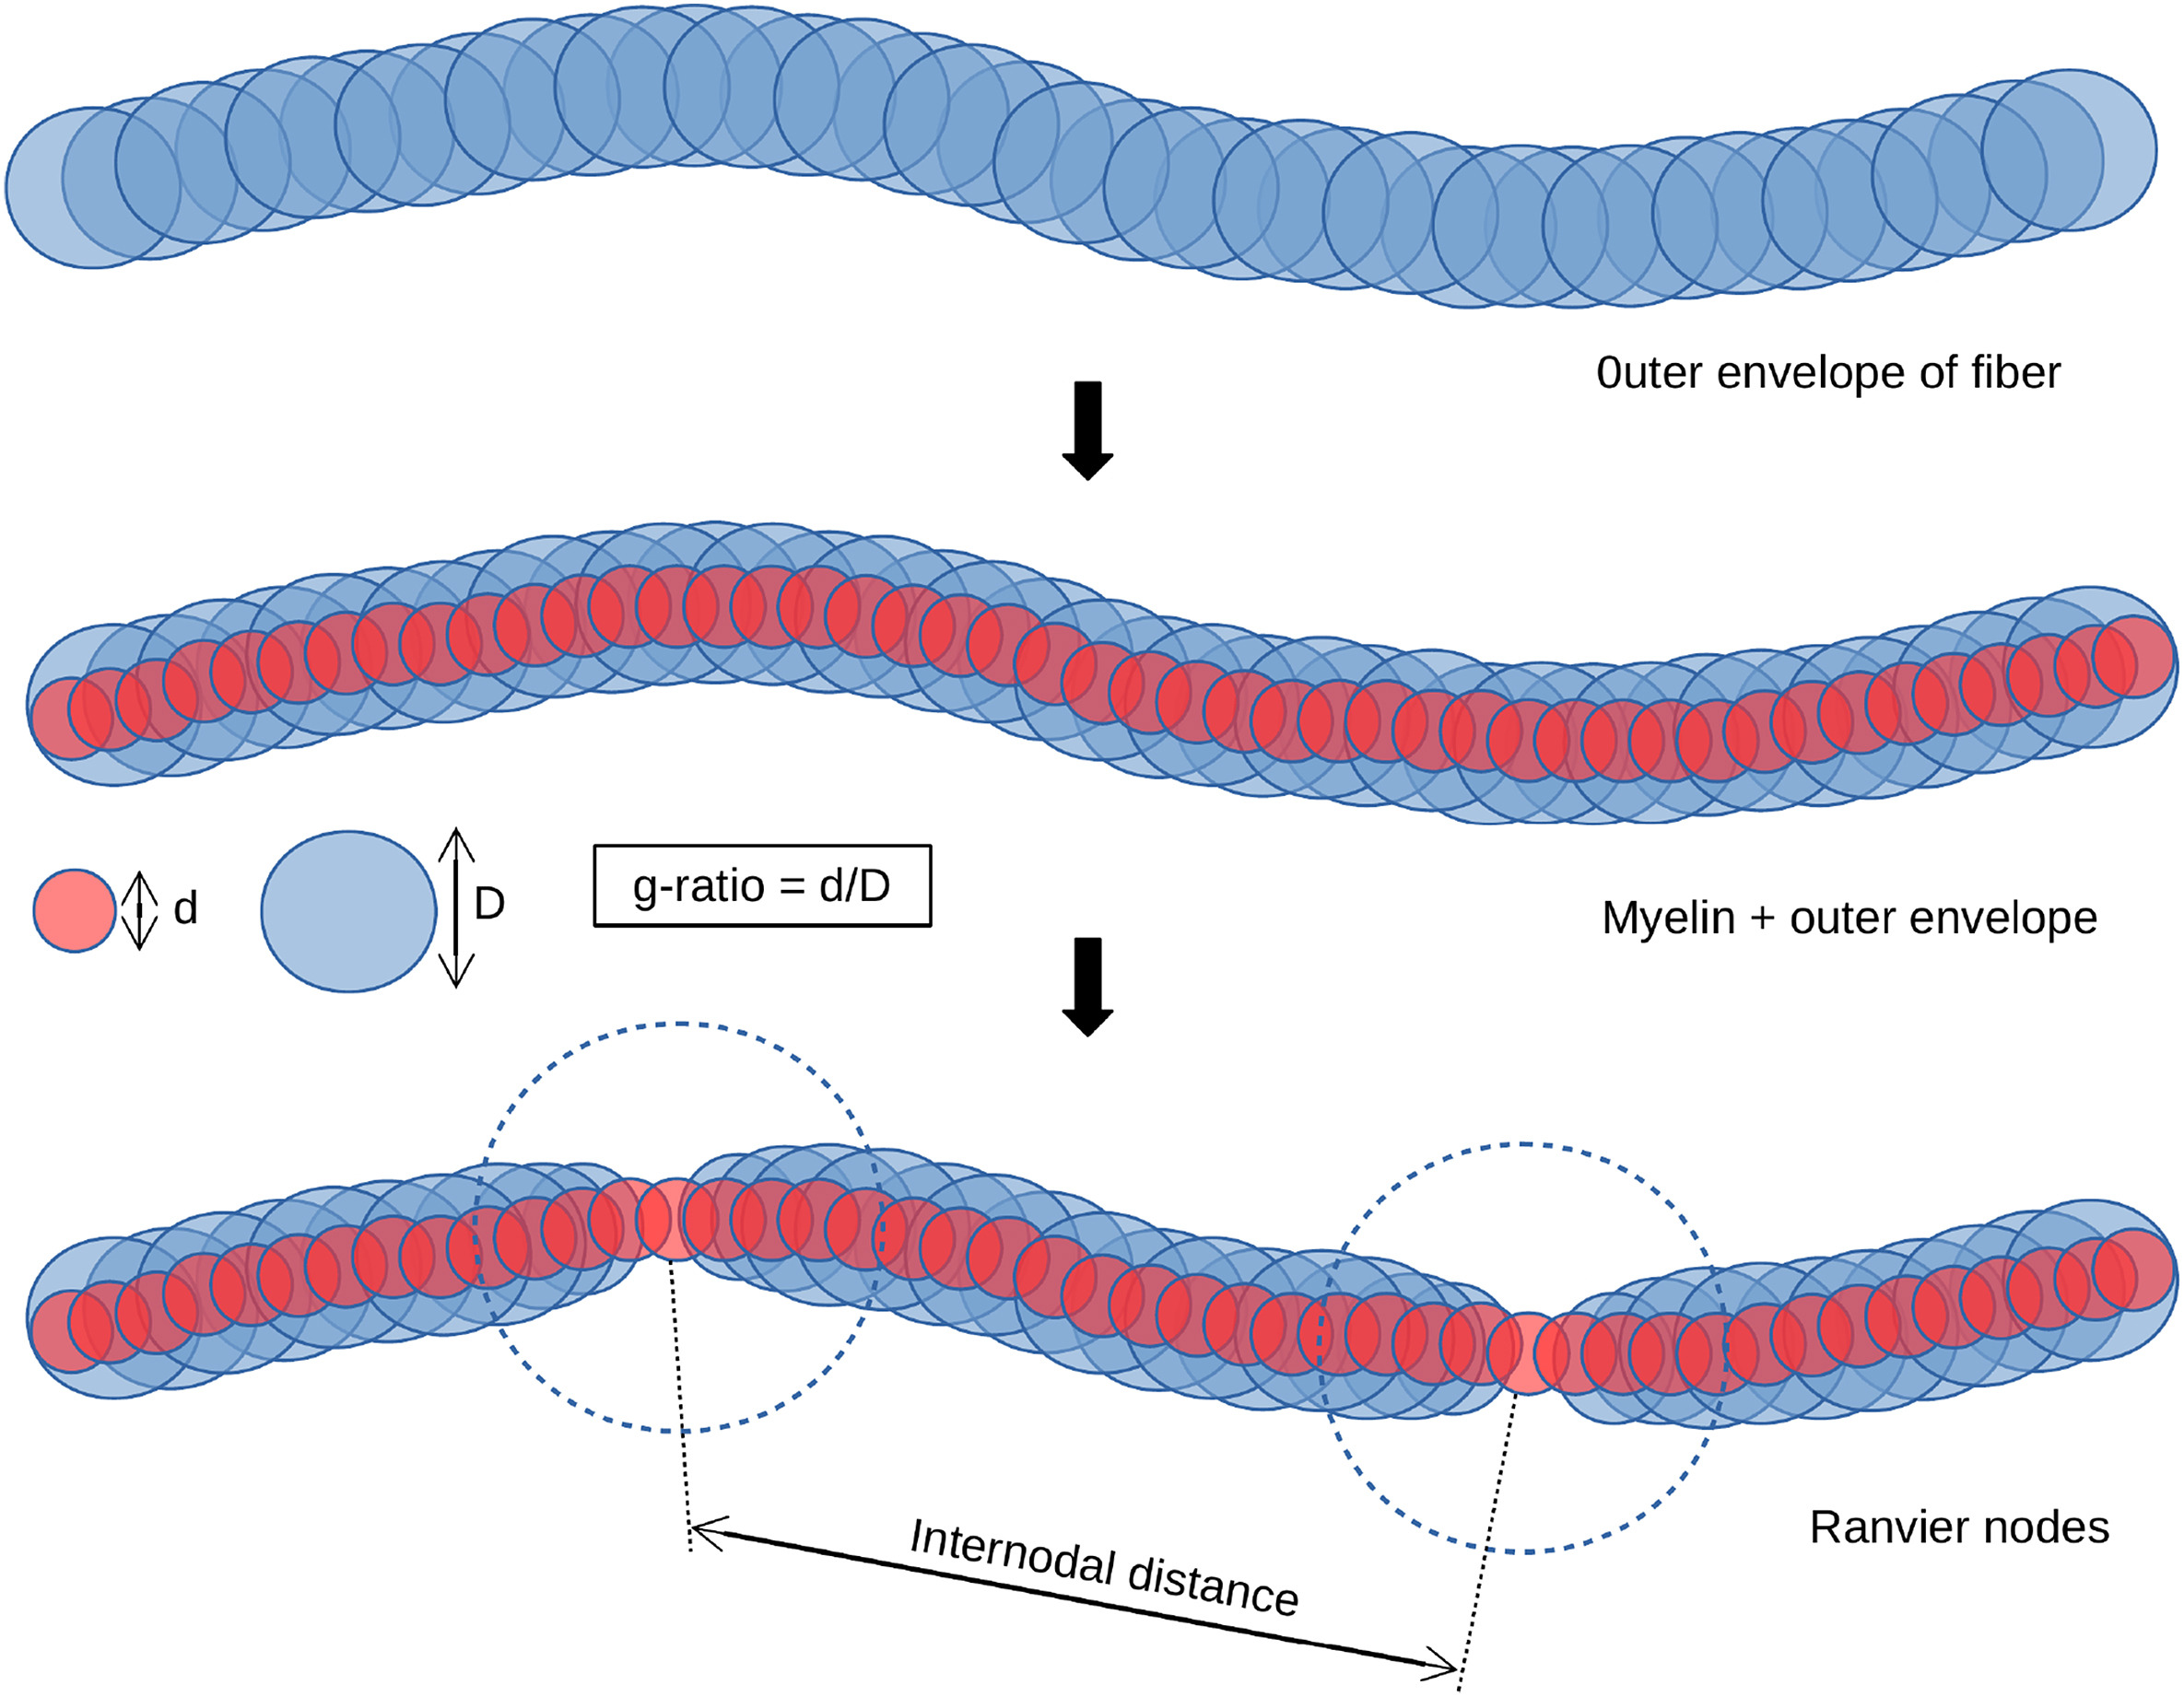
\includegraphics{gfx/model/medusa/4.jpg}
%     % }
% 	\caption{4 \cite{Ginsburger2019}}
% 	\label{fig:model:medusa_4_org}
% \end{figure}
% 
Since all objects are represented as a collection of spheres (see \cref{fig:model:medusa_4})
\begin{align}
    \mathcal{S} = \{ (x_i,y_i,z_i,r_i) : i \in \{0, 1, ..., n_\text{objects}-1\}  \} 
\end{align}
% 
, a collision is present if (VCS !!!)
% 
\begin{align}
\begin{split}
d<r_i+r_j\\
d = \abs{\vec{p}_i - \vec{p}_j}
\end{split}
\end{align}
% 
However since neighboring spheres in one fiber are colliding for a densly populated fiber, they have to be excluded if
\begin{align}
\begin{split}
d(i,j) &\leq  r_i + r_j\\
d(i,j) &= 
\begin{cases}
\sum_{n=i}^{j-1} \abs{\vec{p}_n - \vec{p}_{n+1}},& \text{if } j-i \geq 1\\
0 & \text{otherwise}
\end{cases}
\end{split}
\end{align}
% 
Spheres inside cell bodys are not checked for collision, since their volume aproximate? the volume of the cell.
\\
% 
The calculation of collisions is done via the GPU architecture. For this a first implementation was written with the \name{AxisAligedSortedSearch} \cite{Karras2012}. It sorteds the spheres along one axis, \eg{} x-axis, x-axis, and search for each sphere the fist and last possible collision on this axis:
\begin{align}
\begin{split}
\mathcal{C}_i = \{ s \in \mathcal{S} \mid \abs{s_i.x - s_j.x} < r_i+r_j \}
\end{split}
\end{align}
% 
\begin{lstfloat}[!t]
	\lstinputlisting[style=cpp]{code/medusa.cu}
	\caption{Pseudocode of \acs{MEDUSA} collision checking.}
	\label{alg:medusa_collision}
\end{lstfloat}
% 
The above described algorithm is currently used for volumes $\approx \SI{200}{\micro\meter}$. For this volume size the algorithm is for the current use fast enough. However, more advaned algorithm exist wich can be applied here (\eg{} \name{BoundindBoxHierarchy} \cite{Karras2012}).
% 
\begin{figure}[!t]
    \centering
    \resizebox{0.95\textwidth}{!}{
    \includegraphics{gfx/model/medusa/8.jpg}}
	\caption{8 \cite{Ginsburger2019}}
	\label{fig:medusa_8}
\end{figure}
% 
\begin{figure}[!t]
    \centering
    \resizebox{0.95\textwidth}{!}{
    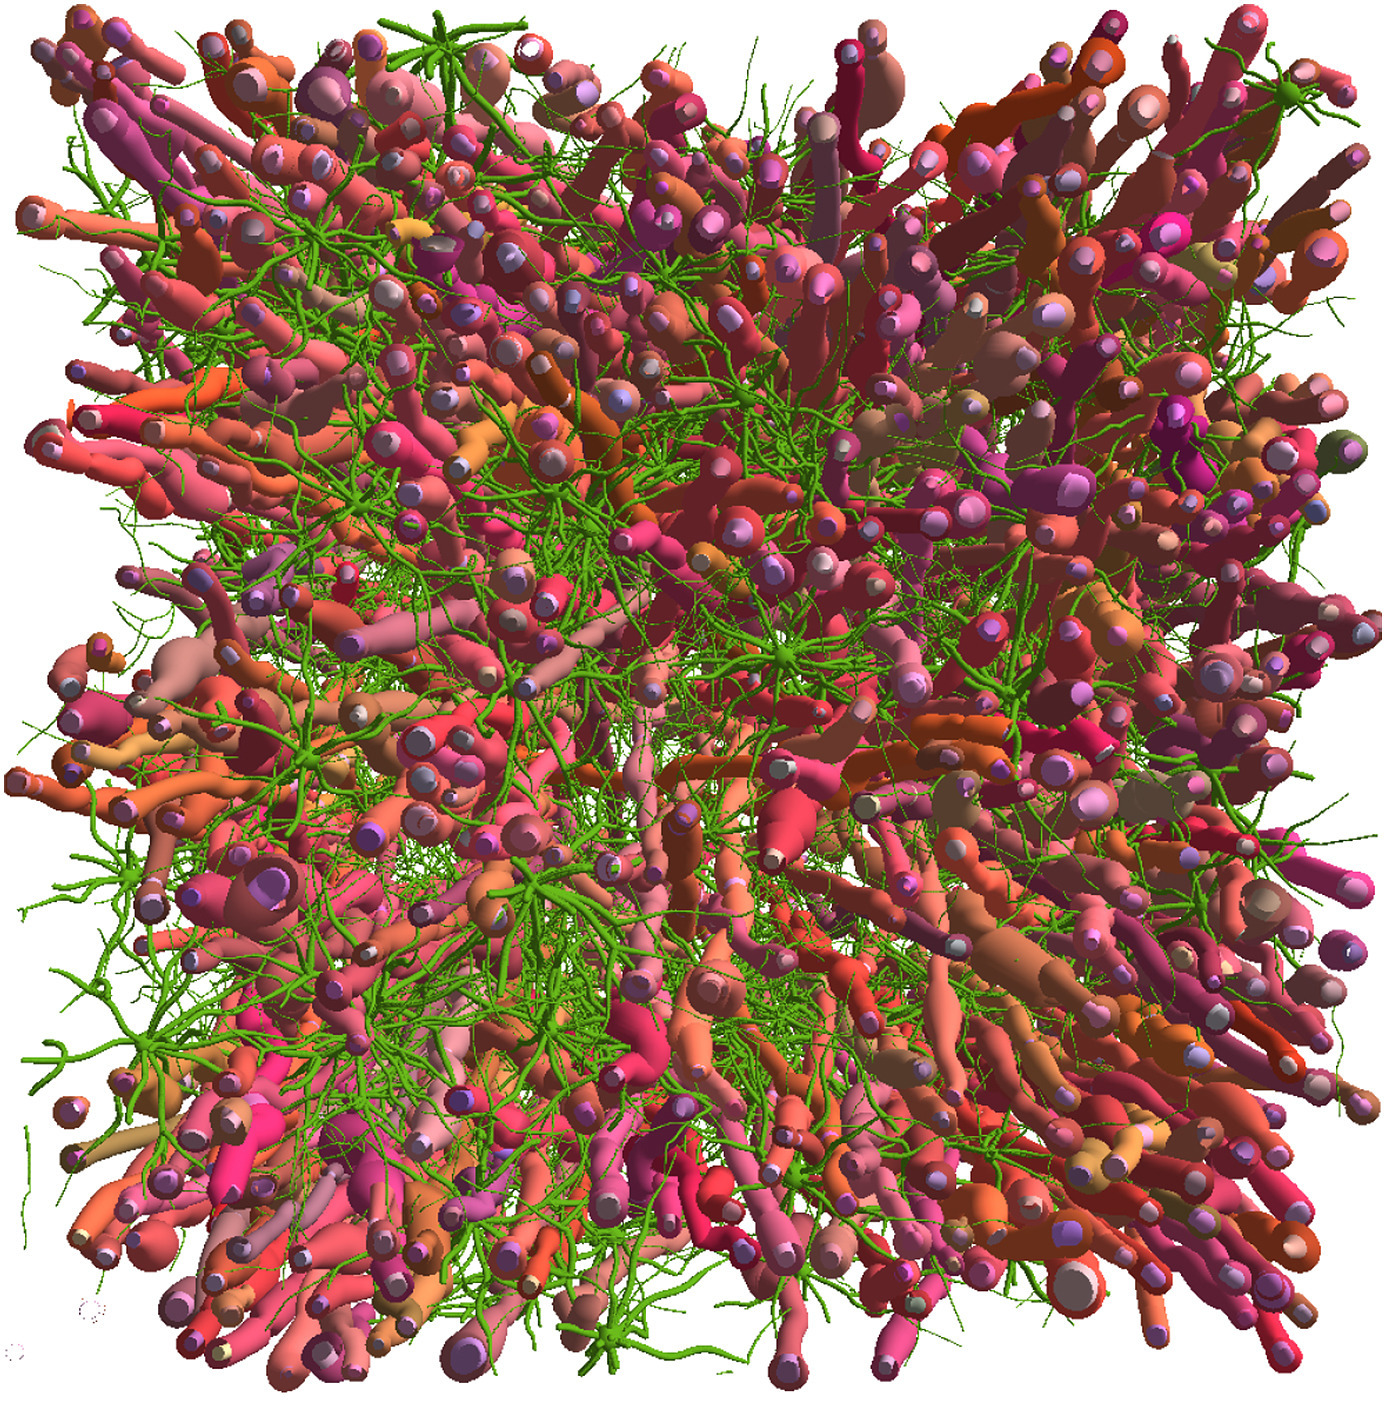
\includegraphics{gfx/model/medusa/11_.jpg}}
	\caption{11 \cite{Ginsburger2019}}
	\label{fig:medusa_11}
\end{figure}
% 
% 
% 
% 
% 
% 
% 
%
% Neurospin works with \ac{dMRI} signals.
% One focus is on the analysis of the fiber architect of the human brain.
% \ac{dMRI} is here quite handy since it is currently the only technique to allow in-vivo measurements to analyse the orientation of white matter tracts. Another importance is the availability of \ac{MRI} machines in almost every hospital in the western civilization.
% Although their resolution is with \SIrange{1.5}{3}{\tesla} limited.
% However, Neurospin is equipped with a mordern \SI{7}{\tesla} \ac{MRI}.
% This makes it possible, including higher measurments times on post mortem brain tissue, a \ac{dMRI} resolution up to \SI{200}{\micro\meter}.
% This makes it possible to allow \ac{3D-PLI} to verify and enhance the analysis of current developed tractography data. 
% %
% Along this works they developed a simulation tool (name) which is computing a Monte-Carlo simulation on the diffusion process in virtual tissues.
% Therefore, for simulations of the \ac{dMRI} signal in the brain, geometric models of nerve fibers as well as nerve cells are required.
% %
% The common goal was, due to a work packes inside the \ac{HBP}, the development of a common general purpose tool to build a geometrical library of nerve fiber configurations.
% Therefore it was decided to work based on the first approaches \cite{Ginsburger2018}.
% %
% \begin{quotation}
% We design a novel white matter numerical phantom generation algorithm which constructs biomimicking geometric configurations with few design parameters, and enables to control the level of disorder of the generated phantoms. The influence of various geometrical parameters present in white matter, such as global angular dispersion, tortuosity, presence of Ranvier nodes, beading, ...
% \end{quotation}
% %
% It is therefore qualified to generate a large database or library of parameter controlled white matter volumes.
% %
% \paragraph{differences:} 
% \begin{itemize}
%     \item All objects are aproximated with spheres.
%     \item Statistical ... of tissue
%     \item diffusion specific parameters
%     \item pathological changes like axon beeding
% \end{itemize}
% 
% \section{Conclusion}
% This allows a user to specify any initial configuration and reaching a collision free model, which, depending on the initial overlap, follows the initial geometry.
% The disadvantage obvious is that the configuration has to change.
% However since biological tissue is deformable and not "caotic" itself, it follows its natrual behavier.
